
\chapter*{About this project}
\paragraph{Abstract:}
This paper proposes a new phone application that consists of numerous features to support third level students. These features include a fully customizable timetable, a countdown timer to exams and deadlines, Google maps feature that highlights useful locations around the local area and an augmented camera function which places an arrow on the camera screen that points towards a selected location. The primary technologies used were Android Studio, SQLite and PostgreSQL. The features can be accessed 24/7 and effortlessly by any user. This report will discuss the process of making such an application and the development of each feature to correspond with both students’ and institutions’ administrative concerns.
 
\paragraph{Authors:}
This project was developed by two 4th year development students, Aaron Flanagan and Ciaran Brennan, as part of our Bachelors of Science honours degree in Applied Software Development.

\chapter*{Acknowledgements:}
We would like to acknowledge and thank Damien Costello for supervising this project. His expert advice and support helped guide this project to completion. We would also like to acknowledge the Department of Computer science and Applied Physics for making this possible and helping us by providing support and any tools that were needed during the development.

\chapter*{Running this project:}
This project can be found on GitHub using the link below.
It contains a small ReadMe file on how to download and run the application. The GitHub repository holds all the classes and native android files created and used by Android Studio to compile and run the project. Your computer or laptop must support virtualization; this can be checked by attempting to install Intel's hardware accelerator software or by checking in the task manager of your machine. If your machine does not support it you will be unable to run the emulator; instead you must plug in an android device with developer options enabled. This varies between devices so you must check how to enable them for your specific device.
\paragraph{GitHub:} https://github.com/AaronFlanagan20/CollegeEssentialsApp.git

\chapter*{Previous Research}
The original idea for this project was to develop a facial recognition music application. The application would begin by capturing an image of the user's face and running a mood capturing algorithm to determine the user's mood, and it would then generate a music file list based on the users' mood. This projects foreground was going to include an animated graphical user interface through the use of the JavaFX library made available by Oracle ~\cite{javafx}. The background would be running a facial detection program that was described by the OpenCV Team~\cite{opencv}. This algorithm was going to be built upon to include facial recognition as it only produced facial detection by displaying shapes around the user's face, however a feature extraction algorithm was required to complete this, which because an insurmountable problem, the choice had to be made whether to change the language or the idea for the project. The decision to begin afresh was informed by our competency in Java over other languages available and due to it being a preference. The reason being we spent weeks of research and study involving different approaches of facial recognition and feature extraction algorithms, only to discover there was no Java binding libraries to OpenCV or resources that we could use. After a week of searching nothing was found that could help us, but because it was still early into the year the project idea needed to be changed as to avoid further problems and time delay. At this stage the project time-line was cut short by three months.

\chapter{Introduction}
“Tech will transform from something we actively use to a more seamless integrated experience that is ‘on’ all the time” ~\cite{nodes}. This is becoming very apparent on university campuses today. It is very unusual to find a student without a personal device such as a smart phone, tablet or laptop. Popular deals with network providers often ensure individuals are connected to 3G or 4G technologies on almost a 24/7 basis, meaning demands for applications to make life easier are only increasing. However, as Corlett et al points out, most applications are designed for an office environment and are not ideal for students’ concerns about time management, revision and lecture attendance ~\cite{corlett}. Creating a student-centric application will address gaps in the current market. Our research of existing products indicated that while there were numerous applications for timetables and notes, none had these features integrated into one, nor were they institution specific. We envisioned our finished product having many reliable ways to track and record information in any educational facility to address common concerns of students.

It was decided to create three primary functionalities, with the possibility of adding more, time permitting. We wished to create a timetable option, with use of a database to ensure the students' data is saved. To help new students navigate the campus, an augmented reality camera overlay would be implemented. Using the Google Maps API would allow the user to locate the college and any notable stores or locations surrounding the educational facility. To aid in time management, students could use customisable assignment countdown timers, colour co-ordinated to reflect the time for study that is left. 
We envisioned the finished product having many reliable ways to track and record information in any educational facility. When the plan was formulated for the new student application, research into the current market was done to see what was already available. We noticed that there are many applications with timetables or notes for phones and tablets, but none that contained all of these sections integrated into one application, or that were institution specific.
 
This report will contain a breakdown and give an in-depth explanation to how the project was approached and developed, the different software and technologies used, an evaluation of the final product and notes taken about each feature and where they can be improved. The following sections will be discussed about the application:
\begin{itemize}
\item Methodology: An explanation of the production approach taken to developing the individual features of the application and how they were developed within the project time limit.

\item Technology review: This section contains details of the various technologies used, both hardware and software. It explains how the project uses each component and gives an explanation to why this particular system/software was used and what is was used for.

\item System design: This section describes the projects architecture, how each aspect was designed to work.

\item System Evaluation: This section is an evaluation of the deliverable compared to the initial design and provides a list of improvements that could be made.
\end{itemize}

Our personal goals include improving our technical capabilities and soft skills useful for the workplace such as communication, team-work, contributing and designing commercial projects. This projects goal is to make life easier for students as best it can and the discussed topics are certainly a good beginning to a useful application. When the project is finished we want to be accustomed to android application development as this is a vastly growing area in the information technology industry and also develop the ability to adapt overcome challenges in a calm and collected fashion.

\chapter{Methodology}
\section{Planning}
We created a project plan to assign tasks and manage our time on the project. This included scheduling meetings, deciding on what software to use, what methodology to undertake and how to test it appropriately. Resulting in that was the creation of a project work flow chart to create a timely estimate of the duration each feature will need and take into account our responsibilities with other projects and reports. The project work flow otherwise known as Gantt chart was developed to display everything that was required and how long was available to complete it. The section that assigns each individual developer to a particular area or feature was left blank because the list of features was not particularly large enough to warrant a seven month time frame, not taking into consideration extra functionality, and it was more beneficial to work as a pair due to the methodology taken. See Figure 2.1. The platform used to develop the project now had to be decided. The three candidates available were: Android, IOS and Windows. IOS was not chosen because of lack in resources. To develop for IOS an Apple computer or laptop was essential and we had no access to one. Android was also favoured over Windows because it was more familiar and Android devices are more popular in the market.

\begin{figure}
	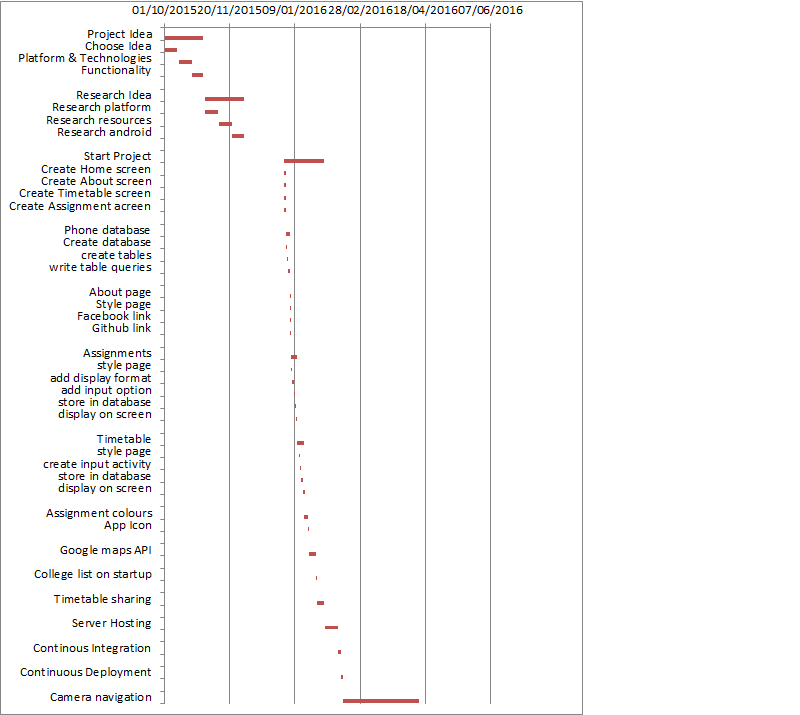
\includegraphics{img/gannt.png}
	\caption{Project Work Flow}
\end{figure}

\pagebreak
\section{Software Methodology}
We decided this project would be developed based on agile methodologies. "Agile methodology is an alternative to traditional project management, typically used in software development. It helps teams respond to unpredictability through incremental, iterative work cadences, known as sprints "~\cite{agile}. The traditional waterfall approach was not taken due to its limitations put on each phase of the project. Each section had to be completed in sequential order and time did not permit backtracking if a problem arouse. Instead an incremental approach was taken. 

Meetings were held to discuss which feature to begin development on, conduct research on previously made work and read through the Android documentation to find relative libraries available. This meant that each feature could be developed regardless of how long was required to complete it and various approaches could be taken if needed. One feature may have taken a week at most to develop allowing more time to improve it, this was not the case though, while the next might have taken far longer to complete. It also allowed for more research and the ability to develop up-to date documentation and code during the development of each feature. If the code had to be re-factored or a different approach needed to be taken that differed from the pre-determined plan outlined at the beginning of this project, time permitted the change and it was documented. During the development of that feature however, an iterative approach was taken. Each developer would plan, develop and test the feature and report back to the original documentation to evaluate it. The same process would iterate until the feature was eventually finished and tested.

Toward the end of each features final cycle a meeting was held to discuss and evaluate it with the supervisor. We discussed ideas on how to improve it or whether to move on to the next task on the list. If time allowed it, improvements were going to be made and further research was done to find what was available, this included previously done work and reading through Androids documentation. Otherwise the feature was closed off and cleaning and testing the code began. The finished updates were then pushed up to the GitHub repository and merged in with all the previous project code and resources.

\pagebreak
\section{Testing}
As mentioned above towards the end of a features cycle, some testing was performed before moving on. This was to insure that the project code did not contain any bugs or errors unseen during the development. This project used three forms of testing. The testing began with Gradle, A tool built into Android Studio and either Gradle or Maven can be selected to formulate the project build. Gradle is a project build automation tool used to compile, test and run Java, C/C++ Native, Android, Python, Hadoop and many more different project types and to slow down build time and code freeze ups ~\cite{gradle}. It complies and runs the project within Android studio on an emulator or installs an Android application package (apk) file to a connected device. This insures that no errors will be thrown at compile time and that the Android apk file will install correctly on the hosts phone without causing any problems. 

Gradle was used to run and test the application however unit tests for the application were written using JUnit. JUnit is "A unit testing framework which is a central element of the Extreme Programming (XP) testing practice."~\cite{junit}. JUnit was used to test the actions of components in the application to check if they performed in the manner they were intended to, for example if a pop-up box is programmed to instantiate itself on the press of a button, a unit test will perform this action and monitor the outcome. The test will return true if the desired outcome is preformed correctly, otherwise it will fail.

Once a commit was pushed up to GitHub it went through CircleCI, CircleCI is a cloud platform used for continuous integration. Every time a commit was pushed up to the repository on GitHub, CircleCI would pull down the commit and run a selection of tests on the new changes. This was done by creating a circle.yml file and adding in the execution command for Gradle: chmod +x gradlew. If the commit passed the test, it was integrated with the rest of the project on GitHub. If it failed, it would not be integrated until the problem was fixed via another commit to update and fix the changes or revert the commit to remove the changes.

\chapter{Technology Review}

\section{Android}
This project was developed for the Android operating system. It was decided that Android Studio was going to be used because android support was stopped for Eclipse now that is uses the IntelliJ platform, which it was built on top off. Android Studio is the optimum integrated development environment available for this application, as it was created and is owned by Android, meaning compatibility is not an issue. "Android is the customizable, easy to use operating system that powers more than a billion devices across the globe — from phones and tablets to watches, TV, cars and more to come"~\cite{android} and Android Studio allows for full access to these customizable features. Android is currently owned, founded and created by Google. It is a Linux-based system and uses Java as its native language along with XML. It combines all that Java has to offer with some custom made Java objects that Android use to interact with the UI component of an application like a TextView or ListView. It's complete, modular and consistent. It makes use of the full operating system the device is running and provides high level APIs for all tasks. This is due to its four layer architecture consisting: Linux Kernel, Libraries and Runtime, Application Framework and then the Applications layer ~\cite{androidarch} Figure 3.1. From a developer and users stand point it is powerful, smooth and really responsive ~\cite{androidsystem}. Each section of the application is called an activity. An activity is defined by a layout file that is in form of an XML document, discussed in the next section. These activities all perform independently from each other unless programmed otherwise. Only one can be open at a time, but another activity can be running in the background waiting for a result of the currently active activity. Below is an example of an activities life cycle: Figure 3.2

\begin{figure}[p]
	\begin{minipage}[b]{0.47\textwidth}
		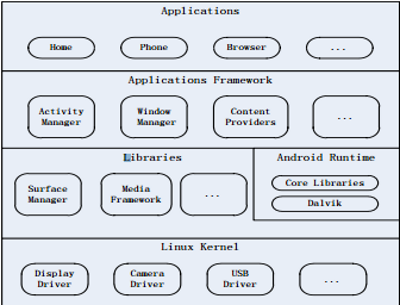
\includegraphics{img/Android-Architecture.png}
		\caption{Android-Architecture ~\cite{androidarch}}
	\end{minipage}
	
	\begin{minipage}[b]{0.47\textwidth}
		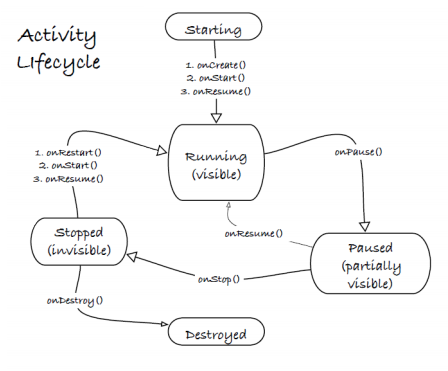
\includegraphics{img/activity-lifecycle.png}
		\caption{Android lifecycle}
	\end{minipage}
\end{figure}

\section{Android XML}
Each element in the layout file represents something that will be displayed on screen. The activity details are specified at the top and then everything is inside a container layout like a FlowLayout our LinearLayout. The element can then be programmatically fetched and used within the class to specify how it should act with an action. For each different aspect of our application, there was a corresponding XML file that created formality among the different components making them all uniform on screen. This factor creates an aesthetically pleasing application, without it each component will float freely and can overlap one another. Each activity, such as the assignment or the timetable activity class, references a standard layout which means just because one activity uses a FlowLayout another cannot use a LinearLayout. Each button, image, list etc.. that is displayed on the screen in our application is controlled by the layout folder containing all the XML documents. When a button is clicked, it triggers the button and checks to see if it is linked to any code within the java folder and executes any runnable code. There is a grid in the timetable XML file that can be filled with any information that a regular timetable would store. This is done by having a toolbar with a ‘+’ on it and when that button is pressed it takes the user to a new layout which has different fields where the module name, time and place can be inserted. Once the correct information is inputted, it is transferred from the current layout to the timetable XML file and displays it on the screen. Below is an example of a layout class that was used for the about page section of the application and Figure 3.2 showing the projects layout files.
 \pagebreak
 \begin{minted}{XML}
 <?XML version="1.0" encoding="utf-8"?>
 
 <android.support.design.widget.CoordinatorLayout
 xmlns:android="http://schemas.android.com/apk/res/android"
 xmlns:tools="http://schemas.android.com/tools"
 android:layout_width="match_parent"
 android:layout_height="match_parent"
 xmlns:app="http://schemas.android.com/apk/res-auto"
 android:fitsSystemWindows="true"
 tools:context="com.collegeessentials.main.About">
 
 <android.support.design.widget.AppBarLayout
 android:id="@+id/assignmentBar"
 android:layout_width="match_parent"
 android:layout_height="wrap_content"
 app:theme="@style/AppTheme">
 
 <android.support.v7.widget.Toolbar
 android:id="@+id/assignmentToolbar"
 android:layout_width="match_parent"
 android:layout_height="?attr/actionBarSize"
 android:background="?attr/colorPrimary"
 android:theme="@style/AppTheme" />
 
 </android.support.design.widget.AppBarLayout>
 
 <RelativeLayout
 android:layout_width="match_parent"
 android:layout_height="match_parent"
 xmlns:android="http://schemas.android.com/apk/res/android"
 android:background="@drawable/background">
 
 <TextView
 android:layout_width="wrap_content"
 android:layout_height="wrap_content"
 android:text="CollegeEssentials aims to help with the navigation and life of a student throughout their college.\n\nDepending on your location, arrows will be displayed on camera directing you to certain sections of the college that you are in.\n\n CollegeEssentials' main features: \n \t1. Navigation around your college.\n \t2. Timetable section to store your classes. \n \t3. A colour coded assignment countdown timer:"
 android:id="@+id/aboutAppText"
 android:textSize="14dp"
 android:textColor="@color/wallet_hint_foreground_holo_dark"
 android:typeface="serif"
 android:focusableInTouchMode="false"
 android:layout_alignParentTop="true"
 android:layout_alignParentLeft="true"
 android:layout_alignParentStart="true"
 android:layout_marginTop="107dp" />
 
 <TextView
 android:layout_width="150dp"
 android:layout_height="50dp"
 android:id="@+id/colourText"
 android:textColor="@color/wallet_hint_foreground_holo_dark"
 android:text="Green is 3 weeks.\nOrange is 2 weeks.\nRed is 1 week.\n"
 android:layout_marginLeft="24dp"
 android:layout_marginStart="24dp"
 android:layout_below="@+id/aboutAppText"
 android:layout_alignParentLeft="true"
 android:layout_alignParentStart="true" />
 
 <TextView
 android:layout_width="match_parent"
 android:layout_height="wrap_content"
 android:text="Please feel free to contact us with your questions"
 android:textSize="14dp"
 android:typeface="serif"
 android:gravity="center"
 android:textColor="@color/wallet_hint_foreground_holo_dark"
 android:id="@+id/contactText"
 android:layout_above="@+id/contactButton" />
 
 <TextView
 android:layout_width="50dp"
 android:layout_height="25dp"
 android:id="@+id/contactButton"
 android:textColor="@color/wallet_holo_blue_light"
 android:text="here"
 android:textSize="16dp"
 android:gravity="center"
 android:layout_marginBottom="26dp"
 android:layout_alignParentBottom="true"
 android:layout_centerHorizontal="true" />
 
 </RelativeLayout>
 </android.support.design.widget.CoordinatorLayout>
 \end{minted}
 
 \begin{figure}[h]
 	\centering
 	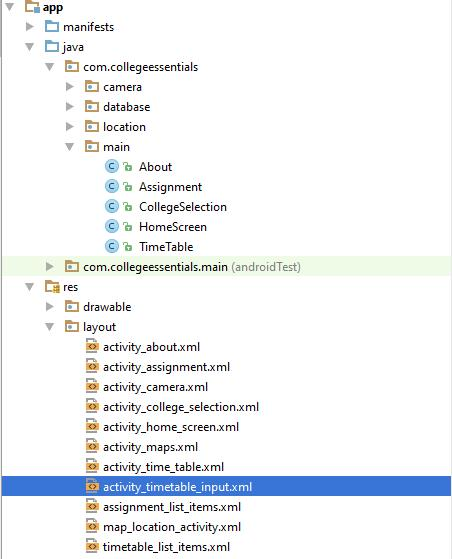
\includegraphics{img/screenshot.jpg}
 	 	\caption{Android studio files}
 \end{figure}
 
\pagebreak
\section{SQLite}
SQLite is an open-source, platform independent, embedded database management system. It is small, fast and free ~\cite{sqlite}. It was chosen due to it's available features and because it is cross-platform. Multiple programs can be written in various languages like Java, PHP or even C++ and they can all access the same database file without compatibility being an issue. Almost all phone vendors and developers support SQLite. The advantages are noted by CHUNYUE in his paper "Research and Application of SQLite Embedded Database Technology" ~\cite{bi}. He describes them as "For its advantages of stability and reliability, fast and high efficiency, portability and so on, which occupies the unique advantages among many of the main embedded database's". He later goes on to describe an embedded database systems architecture and it's characteristics. This report focuses on its advantages to the project and it's capabilities over its low-level functionality. However he gives an in-depth explanation on how it runs in the background and its available functions.
The database file format can be freely copied and moved between various systems without any problems, this also applies to 32-bit and 64-bit systems and big-endian and little-endian. Other key aspects of this is the library and database file sizes are both relatively small. It can be configured to run on a minimal stack space of 4KiB if needed, but usually it is sized at only 500kiB depending on the target platform. The application only has to load as much data as it needs, rather than reading the entire application file and holding a complete copy in memory. Start-up time and memory consumption are reduced as a result of this. It stores everything in one file rather than a pile of files, making it structural and abstract because only databases created in Android are visible to the application that created them. When the application is shut down all databases are destroyed meaning only the needed information can be loaded at runtime. The state of the database is always consistent even in the event of a phone crash or power failure. This is because it uses the atomic, isolated, consistent and durable (acid) features. A SQLite database can also be queried and the data retrieval is much more robust. If you have data that is relative the file allows no association but SQLite helps with that.

\pagebreak
\section{PostgreSQL}
"PostgreSQL is a powerful, open source object-relational database system. It has more than 15 years of active development and a proven architecture that has earned it a strong reputation for reliability, data integrity, and correctness." ~\cite{postgres}. PostgreSQL could be accurately described as an object-oriented system because it includes unique identity for objects, abstract data types, classes (constructed types), methods (functions), and inheritance for both data and functions. PostgreSQL is a external database used for this application that is connected to at runtime and holds the relevant information for each college. Depending on the college selected only the information for that selection will be retrieved and used. The PostgreSQL database used is held and maintained by Heroku, a continuous deployment company. This database was used because originally the project was going to be testes by CircleCI, a continuous integration platform and then be passed onto Heroku for deployment. However the project had files the CircleCI would not except because they should not be checked into a version control system, but Heroku needed. Instead the database was used because it had easy access and it was already set-up to the repository own GitHub. Just like SQLite it is cross-platform, open source, robust, consistent, stable and supports ACID and transactions, which are the basic functionalities of a relational DBMS. Any device or program can connect to it without compatibility being an issue. It supports all functionality most relational database management systems do, but they are known for their data integrity and developer features. Processes like joining very large tables of information are simple. PostgreSQL is slower than MySQL, this is because MySQL focus on optimizing query performance where PostgreSQL allows for more flexible actions like table joins and data clean-ups or using storing procedures. They focus more on the functionality and less on performance, which can be a big downfall for responsive software and websites.

\chapter{System Design}
\section{Server connection}
The first page of the systems design is the CollegeSelection activity. This consists of a ListView object that contains a list of colleges in the country. Once a college is selected the application creates a database with the college's name using SQLite. It makes a connection to Heroku's PostgreSQL database to retrieve the binary data of an image that corresponds to the chosen college and display it on the HomeScreen activity. Android uses a UIThread to handle all the on screen displays and actions, this is the main thread. However Android do not allow networking actions on this thread, a separate thread must be started and ran in the background. This was not possible because the Heroku connection needed to be made to continue. To tackle this problem, the main UIThread is forced to wait for the connection thread to finish. This is not the best way to handle the problem but it served as a temporary solution until another could be found. The connection was made as follows:

\begin{minted}{java}
try {
	connect.start();//start thread
	connect.join();//forcing UI thread to wait until connection is complete
}catch (InterruptedException e){
	e.printStackTrace();
}
\end{minted}

The connect thread created a Heroku connection which in turn called the connect method from its constructor. The Thread.join() statement is forcing all other Threads to wait until it has finished. Below are two screen-shots of the application, while Figure 4.3 describes the flow of events that take place.

\begin{figure}[!b]
	\begin{minipage}[b]{0.47\textwidth}
		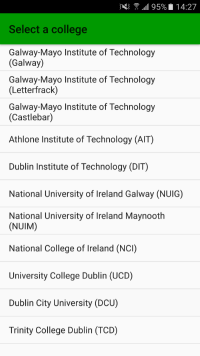
\includegraphics{img/collegeselection.png}
		\caption{CollegeSelection activity}
	\end{minipage}
	\hfill
	\begin{minipage}[b]{0.47\textwidth}
		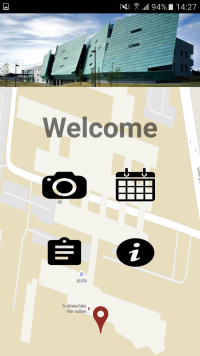
\includegraphics{img/homescreen.png}
		\caption{HomeScreen activity}
	\end{minipage}
\end{figure}

\begin{figure}[!hb]
	\centering
	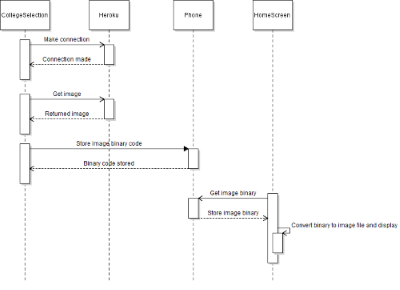
\includegraphics{img/heroku-connection.png}
	\caption{Connection to Heroku sequences}
\end{figure}

\clearpage
\section{Database Technology}
"SQLite is a software library that implements a self-contained, serverless, zero-configuration, transactional SQL database engine. SQLite is the most widely deployed database engine in the world"~\cite{sqlite}. This database management system is independent and available on all mobile platforms. It uses the database query language SQL to insert, delete, update and query database tables made on the users phone and stores information relevant to the application. In Android two objects are used to create and maintain them, SQLiteDatabase exposes methods to manage a SQLite database and SQLiteHelper is a helper class to manage database creation and version management. The application contains three stand-alone tables: Timetable, Assignment and Markers. Timetable contains three columns: module name, room number and teacher name, assignment contains two columns: subject name and the due date. Marker contains three columns: marker name and the longitude and latitude of the selected place in the Google maps section.\newline

\begin{figure}[h]
	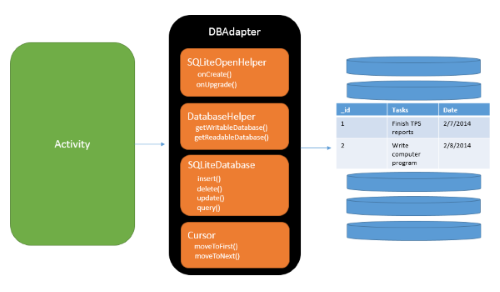
\includegraphics{img/Android-SQLite-Overview.png}
	\caption{SQLite objects}~\cite{using-the-sqlite-database}
\end{figure}

\section{Timetable activity}
The Timetable class of the project creates a screen of TextView objects in the form of columns and rows that represent the days Monday-Friday and times 9:00am - 6:00pm. By clicking a TextView box or by clicking the plus icon in the top right corner a new activity begins to enter in the subject, room, teacher, day and time. This all gets stored in the Timetable table of the database. On creation the class loops through the parent layout and collects all TableRows in it. Tt then loops through every TableRow and selects all the TextView's each of them contain. It creates a temporary TextView object sets it's allowed boundaries and calls the paintTimetable() method. See code snippet getAllTextViews().

This method takes the TextView as an argument, calls the getIDName() method and retrieves the ID in the form of day-time and checks the database for any information it may contain. In the unlikely case the view does not have an ID, it will just return a blank string. A Cursor object is used in Android to loop through the database and store string variables of the data in each column. A check is done to see if the TextView's day and time have any information stored under it and if so it sets the text to it and paints it on screen within the TextView's specified boundaries. See code paintTimetable()
\pagebreak

\begin{minted}{java}
private void getAllTextViews() throws Exception {
 for(int i = 1; i < layout.getChildCount(); i++){//loop through parent layout
  if(layout.getChildAt(i) instanceof TableRow) {//get every child that's a TableRow
   TableRow row = (TableRow) layout.getChildAt(i);//create temp TableRow
   for(int x = 1; x < row.getChildCount(); x++){//loop through temp TableRow
    if(row.getChildAt(x) instanceof TextView){//get every TextView in temp TableRow
     TextView temp = (TextView) row.getChildAt(x);//set child to temp
 	 temp.setOnClickListener(this);
	 temp.setMaxWidth(temp.getWidth());//set size's
	 temp.setMinWidth(temp.getWidth());		
	 temp.setMaxHeight(temp.getWidth());
	 temp.setMaxHeight(temp.getWidth());		
	 paintTimetable(temp);//fill child with details stored in database
    }
   }
  }
 }
}

private void paintTimetable(TextView view) throws Exception {
 String id = getIDName(view, R.id.class).toLowerCase();//pass in an object and get it's id
 String[] search = id.split("_");//split day from time (MON) _NINE
 
 Cursor c = ad.returnTimetableData();//return all data from  database
 
 if(c.moveToFirst()){
  do{
  // Collect each rows data
  String module = c.getString(0);
  String room = c.getString(1);
  String teacher = c.getString(2);
  String day = c.getString(3);
  String time = c.getString(4);
 
   if(day.equals(search[0]) && time.equals(search[1])){// if day = "mon" and time = "nine"
    view.setText(String.format("%s\n%s\n%s", module, room, teacher));//paint details on screen
   }
 
  }while (c.moveToNext());//move to next row in database
 }
}
\end{minted}

\begin{figure}[!tbp]
	\begin{minipage}[b]{0.47\textwidth}
		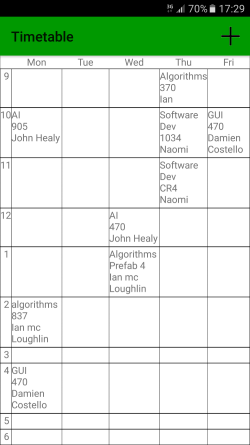
\includegraphics{img/timetable.png}
		\caption{Timetable activity}
	\end{minipage}
	\hfill
	\begin{minipage}[b]{0.47\textwidth}
		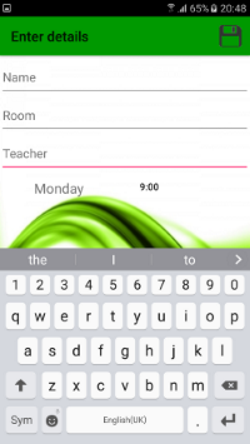
\includegraphics{img/timetableinput.png}
		\caption{TimetableInput activity}
	\end{minipage}
\end{figure}

\clearpage
\section{Assignment activity}
The assignment activity creates a ListView that holds all of the users current assignments. Three input options are available: A textbox for the assignment name, a timepicker widget to select the time and a calendar widget for the date. Each ListView item consists of two TextView's for the name and count down timer and a button to delete the assignment once it expires. On creation, the ListView is initialized and the database is looped through and all current assignments are returned and stored in a list. This list contains the Display(Code snippet Display) object that was designed to be a Data transfer object to hold all the data from each row. The ListView is then handed a custom ArrayAdapter called Countdown Adapter. The CountdownAdapter starts the timer that provides it with the continue down effect and sets all the views on screen(Code snippet getView()). To do this it uses the custom ViewHolder that was built to create the on screen elements and convert the time from milliseconds to days-hours-minutes-seconds(Code snippet timeDiff) and update the information and TextView with the new time.

\begin{minted}{java}
private class Display {
 String name;
 long expirationTime;

 public Display(String name, long expirationTime) {
 this.name = name;
 this.expirationTime = expirationTime;
 }
}
\end{minted}

\begin{minted}{java}
long timeDiff = mDisplay.expirationTime - currentTime;
if(timeDiff > 0) {
 int seconds = (int) (timeDiff / 1000) % 60;
 int minutes = (int) ((timeDiff / (1000 * 60)) % 60);
 int hours = (int) ((timeDiff / (1000 * 60 * 60)) % 24);
 int days = (int) ((timeDiff / 1000) / 86400);
 tvTimeRemaining.setText(format("%d days %d hrs %d min's %d sec", days, hours, minutes, seconds));
 return days;
}else {
   tvTimeRemaining.setText("Expired!!");
   return 0;
 }
\end{minted}

\begin{minted}{java}
public View getView(int position, View convertView, ViewGroup parent) {
 
 ViewHolder holder;
 if (convertView == null) {
  holder = new ViewHolder();//get our view
  convertView = lf.inflate(R.layout.assignment_list_items, parent, false);//add our list
  holder.name = (TextView) convertView.findViewById(R.id.name);//setup out name
  holder.tvTimeRemaining = (TextView) convertView.findViewById(R.id.timeRemaining);//and time left
  deleteButton = (ImageButton) convertView.findViewById(R.id.deleteButton);
  convertView.setTag(holder);//set our view to hold these
  synchronized (lstHolders) {
   lstHolders.add(holder);//add our holder to the list
  }
 }else {
   holder = (ViewHolder) convertView.getTag();
  }
 
 holder.setData(getItem(position));//set all the data to it
 
 //decide what colour to set based on remaining time
 String daysLeft = getColour(holder.updateTimeRemaining(System.currentTimeMillis()));
 if(daysLeft.equals("red")){
 convertView.setBackgroundColor(Color.rgb(255,0,50));
 }if(daysLeft.equals("orange")){
 convertView.setBackgroundColor( Color.rgb(255,165,0));
 }if(daysLeft.equals("green")){
 convertView.setBackgroundColor(Color.rgb(0,255,127));
 }
 
 return convertView;
}
\end{minted}

\begin{figure}[!tbp]
	\begin{minipage}[b]{0.47\textwidth}
		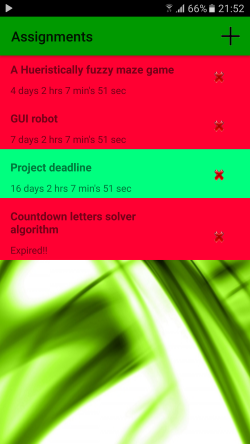
\includegraphics{img/assignment.png}
		\caption{Assignment activity}
	\end{minipage}
	\hfill
	\begin{minipage}[b]{0.47\textwidth}
		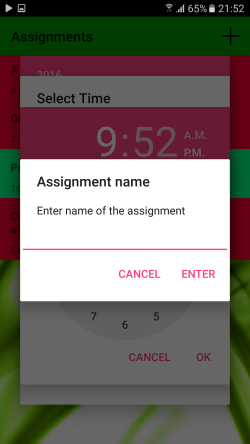
\includegraphics{img/assignmentinput.png}
		\caption{AssignmentInput}
	\end{minipage}
\end{figure}

\pagebreak
\section{Augmented Reality}
Augmented reality creates a layer between the physical world and the digital world. Augmented reality adds graphics and sound to the natural world, through a device such as phone or through video games. This makes users ask questions like what is real and what is computer generated? Augmented reality was included in this project in the form of navigation around the selected college with a rotating arrow. This arrow points towards the location the user wants to go. On start-up of the camera activity the phone will call its camera instance and place a preview on top of it. This means the camera can be controlled and changed without altering the actual camera instance. This is accomplished by extending the SurfaceHolder object in the CameraPreview class and implementing the SurfaceHolder.Callback to receive updates when the surface changes. A SurfaceHolder is an "abstract interface to someone holding a display surface. Allows you to control the surface size and format, edit the pixels in the surface, and monitor changes to the surface"~\cite{surfaceholder}. The DrawView object is then created and added to the preview. DrawView extends the SurfaceView object which is a drawing surface embedded into the SurfaceHolder. You get a reference to the main layout and add the preview to it and then add the draw view on top of that. Like so: 
\begin{minted}{java}
 mCameraPreview = new CameraPreview(this,c);
 alParent.addView(mCameraPreview);
 
 // Create a new draw view and add it to the layout
 DrawView drawView = new DrawView(this);
 alParent.addView(drawView);
\end{minted}

It then allows the camera to be drawn on using the onDraw method within DrawView thus creating the augmented reality effect. The draw method starts by getting the phones location by making a call to the PhoneLocation object. It then sets the point we want to go to, which in the future will be a call to the database. It will then paint an arrow on screen, calculate the degrees between the current latitude longitude point and the desired points and rotate the arrow to point in that direction.
\begin{minted}{java}
@Override
protected void onDraw(Canvas canvas) {
 super.onDraw(canvas);

 canvas.drawColor(0, PorterDuff.Mode.CLEAR);

 loc.getPreviousLocations();//stores last location

 to = loc.getToLocation();
 from = loc.getFromLocation();

 to.setLatitude(53.2831252);
 to.setLongitude(-9.0414227);

 degrees = getDegrees(from.getLatitude(), from.getLongitude(), to.getLatitude(), to.getLongitude());

 canvas.rotate((float) degrees, canvas.getWidth() / 2, canvas.getHeight() / 2);

 //gmit canteen 53.2791608,-9.0105963
 textPaint.setARGB(255, 200, 0, 0);//Colour red - ish
 textPaint.setStyle(Paint.Style.FILL);

 /* Top arrow*/
 textPaint.setTextSize(70);
 canvas.drawText(degrees + "", 1100, 500, textPaint);

 textPaint.setStrokeWidth(20);
 canvas.drawLine(1250, 100, 1250, 400, textPaint);

 textPaint.setStyle(Paint.Style.STROKE);
 textPaint.setStrokeWidth(2);
 textPaint.setColor(Color.RED);

 Path path = new Path();
 path.moveTo(0, -100);
 path.lineTo(50, 0);
 path.lineTo(-50, 0);
 path.close();

 path.offset(1250, 100);
 canvas.drawPath(path, textPaint);
 
}
\end{minted}

\chapter{System Evaluation}

\section{Assignment Feature}
The assignment countdown timer feature was fully developed and all goals were achieved. The user can enter in the name of the assignment, pick the time it's due at with the clock widget and then choose a date it was due by using a calendar widget. It would then be colour coded to alert the user of how long they had left to complete it. Red meant there is less than a week to do it, orange means less than 2 weeks and green means 3 weeks or more. It functions exactly as it was outlined in the beginning with the colour co-ordination being added as extra functionality. However it does need some added functionality. The ability to change the name of the assignment is a must. If a user enters the name incorrectly and they wish to change it they must delete it and re-insert it again. Also the timer is roughly around 20 seconds to slow meaning after the upload time for the assignment expires the timer is still on the 20 second mark give or take. The timer is converted from the systems nanoseconds to days hours and minutes so it has been a challenge to fine tune the timer to the exact second. The time is converted like so:
\begin{minted}{java}
 long timeDiff = mDisplay.expirationTime - currentTime;
 if(timeDiff > 0) {
  int seconds = (int) (timeDiff / 1000) % 60;
  int minutes = (int) ((timeDiff / (1000 * 60)) % 60);
  int hours = (int) ((timeDiff / (1000 * 60 * 60)) % 24);
  int days = (int) ((timeDiff / 1000) / 86400);
  tvTimeRemaining.setText(format("%d days %d hrs %d min's %d sec", days, hours, minutes, seconds));
  return days;
 }
\end{minted}

\section{Timetable Feature}
The timetable sections are fully complete as outlined in the introduction. The user can click the '+' icon or select a section by tapping on screen and they will be brought to the input activity. Here they can enter their module name room number, lecturer name and can choose what time and day the class is on. The application screen will quickly refresh and display the class. The timetable also resizes it's self accordingly to allow extra view space for one class if any sections around it are empty. It will not take up extra space or favour over another class. There are still extra features that can be added to improve the quality of it. Users could be able to share their timetables with other users by clicking a 'share' button. The application could have a remote ID and the user can send it to the specified ID in XML format. The application can open the XML file read it and populate the database with the information. Also when the user clicks on a certain class, the input section adjust its day list and time picker/widget so the user doesn't have to specify it again on input.

\section{Camera Navigation}
The augmented reality section was not a complete success. It does not fully function according to the outlined plan. The original idea was to have two or more arrows pointing to different locations around the users' selected college. Only Galway-Mayo Institute of Technology was going to be included in the navigation for this project and the remainder were going to be implemented thereafter. Currently only one arrow is present on screen and is not fully functional. It obtains the angle between the users current latitude and longitude points and the designated points. Even this has proven to be quite difficult. The angle tends to be off by a few degrees or by a lot of degrees. It is also unfortunate that there is not many resources in augmented reality made available by outside developers or Androids documentation themselves. Few resources exist showing how to implement the SurfaceView and SurfaceHolder objects but none that are augmented reality specific. This section was a major downfall for the project and it would be advised to allow for extra time to research and practice Android development in order to pursue augmented reality in the future.

\section{Databases}
The database management system used is SQLite and PostgreSQL. This database was chosen for the reason that all mobile platforms support it. This enables the phone to have a certain degree of control on what particular information it receives when needed. PostgreSQL handles all the default information that is stored in each separate section under the different college choices available, such as home screen picture and default Google map markers we have set. The PostgreSQL database requires an internet connection to pull down the information required.On running the application, a college selection menu is activated and the user selects the college that the user is attending. This list feeds in specific information which is stored in a database to the application and information is changed accordingly. A separate database is used to store user defined information such as the timetable, assignments and custom Google map markers the user may have placed which is stored in the SQLite database. The SQLite database does not need an internet connection as it is stored on the application itself within the phone. The database model stores two tables, Timetable and Assignment. The Timetable activity contains three columns room, teacher and subject, while the assignment activity contains two, subject and due-date. With information stored in multiple databases the applications overall size averages around 27.5MB, which compared to a larger scale size application, such as Facebook’s social network, it is miniscule. Facebook’s official application is currently at 365MB. 
A connection is also made to Heroku’s PostgreSQL database to pull down an image of the college stored and the co-ordinates needed for the navigation section. Doing it this way saves memory on the phone instead of each database per college storing the image and wasting memory it retrieves the binary of said image and re-converts it to a bitmap from the main screen every time the application is used and places it on screen. To do this a separate project was made to act as the Heroku maintenance code of the database, also using java. This code is used to test the pushing and pulling of information to the server. Once everything is pushed up it never has to be done again, but the code is then integrated into the project to deal with retrieving the image.

\section{Universality}
A decision to make the application universal was made during the development. All students can use the timetable and assignment features. The navigation section will be constantly updated to allow other colleges to use it. However at the moment the application is only accessible to Android users. Android was chosen because it is consistent, stable, popular and a preferred development platform. However the initial intentions of the project were for it to be available on all platforms. Different technologies exist that allow the application to be complied cross-platform to the IOS operating system for IPhone and Microsoft Windows operating system for Microsoft phones, but this was not accomplished because time ran out. The overall structure of the project will be concrete regardless of the operating system because of the platform neutral technologies chosen. The chosen database explained previously in the technology review of this report is SQLite. SQLite is supported by all mobile platforms as a database choice. The syntax of all the internal queries made in the application will remain the same. However the initial setting up of the database will need to be done through the programming language for that platform. The same concept applies to the college selection, as previously explained Heroku's PostgreSQL database is entirely independent from the applications architecture. The only difference being the driver that enables the connection on each platform. Android uses Java's JDBC driver to connect. This driver will be of no use to the other platforms because IOS is written in either Objective-C or Swift using the ODBC driver, and Windows is written using C-Sharp and uses the ADO.NET driver. This means each operating system specific deployment of the project will need to have its own driver included and the syntax within the CollegeSelection class of the project will have to change slightly to replace the JDBC driver reference with the new one. Each language uses it's predefined driver in order to make a connection to Herokus database and retrieve information based on an SQL query the application makes. This was necessary so the phone doesn't waste memory storing information and images for all the colleges. See Figure 5.1

\begin{figure}[h]
	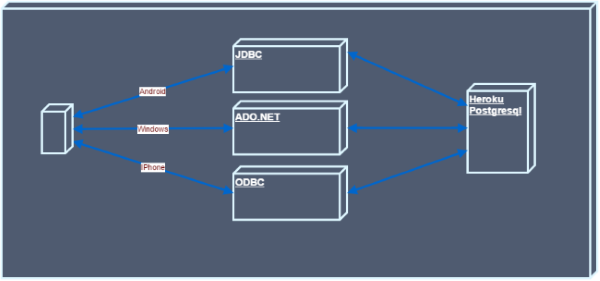
\includegraphics{img/connection-diagram.png}
	\caption{Phone Driver Diagram}
\end{figure}

\pagebreak\section{Improvements}
Each section of the application has areas where improvements could be made if more time was available. Below is a list of possible improvements that can be made in the future for the application in general and each individual section. 
\begin{itemize}
	\item Application: A priority queue added to handle threads because the current implementation creates a lag in the connection.
	\item Application: Add in an instant messenger section for students to talk to one another about their timetables and current assignments.
	\item Application: Add a section that users can personalize it to their preference.
	
	\item Camera navigation: More colleges and universities in the country can be added to the list.
	\item Camera navigation: Better graphics can be used for augmented reality.
	\item Camera navigation: More responsive software to deal with multiple locations within the geo-fencing area.
	\item Camera API: A swap from the deprecated Camera API to the new camera API made available for newer Android SDK's. 
	
	\item Assignment: The ability for users to share assignments across platforms with each other.
	\item Assignment: Section for lecturers to upload assignments and the users can just enrol to that assignment.
	
	\item Timetable: The ability for users to share timetables with each other.
	\item Timetable: Section for colleges to upload timetables automatically and users can download it.
	\item Timetable: Colour code each section of the timetable.
	
	\item Google Maps: Option to view each individual floor of a building being seen.
	\item Google Maps: Provide directions from current location to a marker chosen by the user.
\end{itemize}

\chapter{Conclusion}
We successfully achieved in building an application that helps students organize their college work which is important in achieving the best possible results. A recommendation that we would give for anyone working on a similar application would be to get a larger sample size of different phone types with unique versions of android as component layouts differ between their operating system. Through the use of Android documentation, learning and coding the application did not prove to difficult as there was a vast amount of resources available apart from the augmented reality aspect. We discovered that there is a limited supply of resources in relation to augmented reality android applications so allow extra time for research in that area. We have achieved everything we set out to accomplish in the beginning with the exception of having the augmented reality side not fully functioning as expected. We have, however added extra functionality that was not previously planned such as the Google maps API and deciding to make the application universal in relation to being compatible for various colleges around the country. It was originally outlined to only create the application for the Galway-Mayo Institute of Technology.


